\chapter{Methodology and Work}\label{chap:chap3}

\section{Tool and Subject Selection}

\subsection{Subjects}

To assess the validity of a developed solution, a collection of subjects to test must be collected. While several previous work has compiled collections of merge commits with semantic conflicts, the collection done by Nuno Castanho \cite{kn:nuno} is particularly useful, being publicly available, closely related to our own work, and also allowing us to draw direct comparisons. Most importantly, it aggregates merge instances from both Silva et al \cite{kn:leuson} and Sousa et al \cite{kn:safemerge}, while also providing valuable information, due to the work developed, such as the specific type of conflict present and whether it was detected and correctly tested by UNSETTLE (providing us with a "base truth"). Furthermore, it has compiled a set of fabricated conflicts, which provide simpler isolated examples that can aid us as they should be easier to detect and test.

\subsection{LLM's}

While preliminary work sought to explore ChatGPT and Llama (both CodeLlama and Llama 2), hardware constraints meant we were unable to explore Llama. Bing AI and Bard were also considered, but they were problematic due to very stringent message size limits, in the case of Bard, and generally worse results: Bing AI, for example, could not wait for all the information to be sent, if split in more than one message and thus generated confused responses. ChatGPT, being hosted online for free and with generous message size limits, proved to be the most reliable option. Despite this, many capabalities that could prove invaluable for this work remained locked behind a premium paywall.

\section{Evaluation of ChatGPT's capabilities}

\subsection{Fabricated Examples}

In the initial step of work, we superficially explored ChatGPT's ability to generate tests for an example conflict of Point, where a distance method is altered from euclidean to manhattan in one branch and in the other branch, a move method is changed from using the value 1 for x and y movement to using the result of the distance calculation.

We tested two frameworks, first just asking for a test, with prompts based on the testing indications given by the DSL for the case:

\begin{itemize}
  \item A Dependency Based semantic conflict was possibly introduced in a 3-way merge. Develop a test for the class Point, that covers the methods move() and distance(), without calling distance() directly.
Before the merge, the class under test was: [base Point]
After the merge, it was: [merged Point].
  \item A Dependency Based semantic conflict was possibly introduced in a 3-way merge. Develop a test for the class Point, that covers the methods move() and distance(), without calling distance() directly.
Before the merge, the class under test was: [base Point]
In the branch A it was changed to: [A Point]
In the branch B it was changed to: [B Point]
After the merge, it was: [merged Point].

\end{itemize}

For this, the LLM simply took one version and created tests taking it as correct behaviour. In the first case, for Base and in the second for Merge. This is not ideal, as the first does not allow us to distinguish if the behaviour changed due to merging, or just do to changes in the branches. The latter takes merge as correct behaviour and will thus always fail.

Other tests involved first asking for an explanation if there was a merge conflict there, before asking for a test

\begin{itemize}
  \item We have done a merge on a piece of code.
Before the merge, the code was: [code]

In the branch A it was changed to: [code]

In the branch B it was changed to: [code]

After the merge it was: [code]

Do you believe there could be a merge conflict here? Where? Explain why.
  \item We have done a merge on a piece of code.
  
Before the merge, the code was: [code]

In the branch A it was changed to: [code]

In the branch B it was changed to: [code]

After the merge it was: [code]

Do you believe there could be a merge conflict here? Where? Explain why. Pay attention to both additions and modifications.
  \item We have done a merge on a piece of code code.
  
Before the merge, the code was: [code]

In the branch A it was changed to: [code]

In the branch B it was changed to: [code]

After the merge it was: [code]

Do you believe there could be a *semantic* merge conflict here? Where? Explain why. Pay attention to both additions and modifications.

\end{itemize}

The first two prompts failed. Indeed for prompt ChatGPT only mentioned the changes in move, but even after prompting it to pay attention to distance, it failed to identify the conflict. For both, it seemed to not understand what was being referred to when speaking of conflict, describing all changes as a "conflict". Thus it would say, there is a conflict between whether to use euclidian and manhattan distance and there is a conflict on how the move function works.

The last prompt given, highlighting the *semantic* aspect of the merge conflict, yielded good results, with the conflict being perfectly described, as seen in figure \ref{fig:semconf}. After prompting for a test, it generates an appropriate one: it tests if the move function updates Point appropriately based on the euclidean distance. Thus it fails for base and branch B, where movement is still done with the value of 1, it passes for branch A as there move is based on distance; and it fails in merge, as now movement is being done with the distance calculation, but the calculation is now manhattan.

\begin{figure}
    \centering
    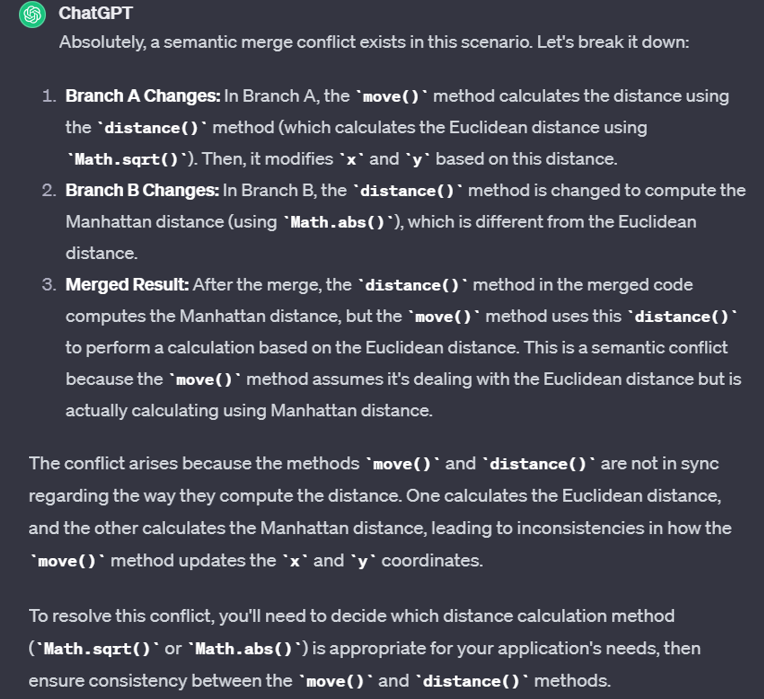
\includegraphics[width=0.75\linewidth]{figures/image.png}
    \caption{ChatGPT description of the semantic conflict}
    \label{fig:semconf}
\end{figure}

In simple fabricated scenarios, where simple conflicts were added to existing software solutions, ChatGPT showed ability to identify and describe the semantic conflict. Despite this, test generation remained complicated and few of the successful identification of semantic conflicts yielded working tests. The final prompt follows.

\begin{quote}
Generate a Junit unit test to identify this semantic conflict, knowing what you do now. The test must compile without errors and require no further alterations. It should require no further dependencies and import all classes correctly.
\end{quote}

While adapted to avoid common pitfalls, the tests generate still suffered from basic issues such as missing imports, which could be mitigated by prompting the LLM for correction automatically. More complex issues of implementation were present, such as calling the base function instead of dependent, wrong usage of construction and function returns, parameter types or unnecessary mocks. Further, when prompting for correction, the LLM often explains that the developer should correct this, thus further work needs to be done to ensure the tool does all the work itself.

\subsection{Real-World Merge Conflicts}

Prompting in real-world examples, or more complex fabricated examples, has produced far worse results. Several refinements were made to the prompts, most significantly: the usage of "git diff" to highlight the specific changes in branch A and branch B, the explanation of the conflict present and the specification of the target method where the conflict is evident. These modifications were largely unsuccessful and did not lead to identification of any conflicts.

We also had to reckon with size limits for messages. Thus, when necessary, we started with an explanatory prompt and then fed the information step by step. However, it remained crucial to remind the LLM of the goal in the last message.

\begin{quote}
We have done a merge on a piece of software and introduced a semantic conflict of types: "Update two different dependencies of a method or update one method and concurrently update one of its dependencies" and "Concurrent changes to the same method". I will now show the base commit, the diff in branch A, the diff in branch B, and the final merge version in 4 separate messages. At the end I want you to explain why and where the semantic conflict is present.
\end{quote}

Common issues are confusion between textual and semantic merges, which can be mitigated by clear explanation of what a semantic merge is; hallucinations of features not present in the code or hallucinations of changes where changes were not made; lack of focus on the methods where conflict is evident, despite reiterations; loss of focus when prompt has to be split into several messages. When the tools do understand what a semantic conflict is and what changes have been made to the code, the best description they can give is to point out them out followed by the suggestion that there may be a conflict there, usually passing on the responsibility of identifying and resolving it to the human user, as seen on figure \ref{fig:cantfind}.

\begin{figure}
    \centering
    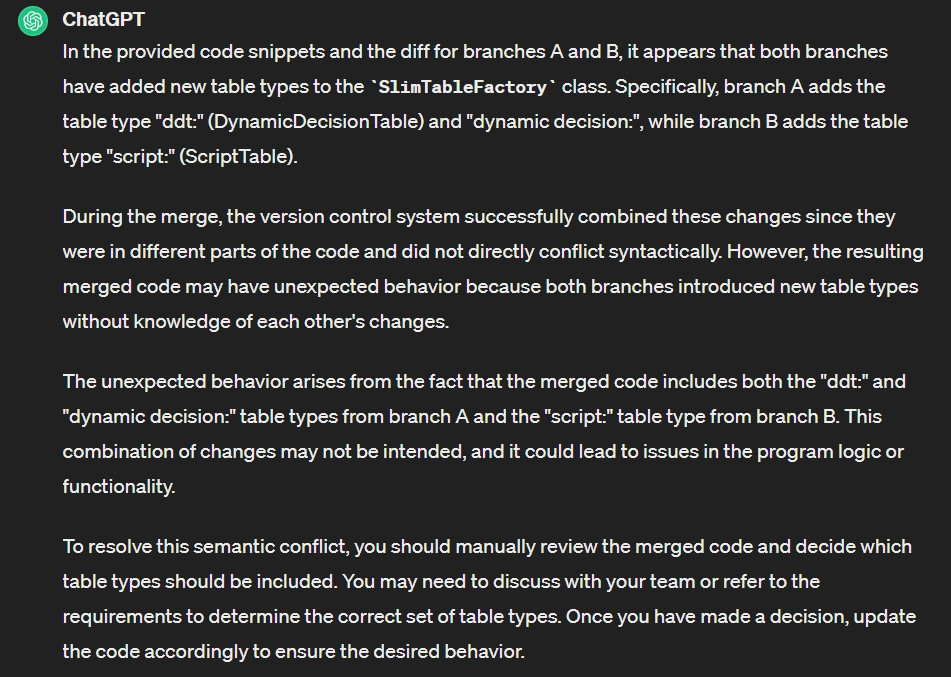
\includegraphics[width=1\linewidth]{figures/almostsemantic.jpg}
    \caption{While nothing said is incorrect, ChatGPT remains unable to identify the conflict proper}
    \label{fig:cantfind}
\end{figure}

While we found that ChatGPT could not identify the semantic conflicts present in real software solutions, in some of Nuno Castanho's fabricated scenarios \cite{kn:nuno}, these were correctly explained. Part of the difference between real-world examples and fabricated scenarios may come down to the information given. The fabricated scenarios were accompanied with a description of the specific semantic conflict present and the changes made perfectly reflected the description, with clear modifications and no extraneous changes. Thus it is possible collecting and offering that information with real-world scenarios may improve the ability of LLMs in this regard, but the higher "noise" of these scenarios may be too disruptive in this regard.

Another factor in consideration is the issue of dependencies, as so far testing had focused on just a unitary class. Given that semantic conflicts can involve interactions between classes and subclasses or other dependencies, it is relevant to provide further information. Initial tests just added one dependency, whether by calling a class methods or due to a inheritance relationship. An example, with the addition of an illustrative example of a semantic conflict follows.

\begin{quote}
We have done a merge on a piece of software and introduced a semantic conflict of type Parallel Changes in Method.

Semantic conflicts occur when concurrent and syntactic-correct changes in different regions of a source file or different files cause the software system to misbehave. For example, suppose there is a Java class `Point` with a method `distance()` that computes the Euclidean distance of a Point to the origin and Bob decides to modify `distance()` so it computes instead the Manhattan distance. At the same time, Alice, not aware of Bob's changes, creates a new method `move()` that uses `distance()` to calculate the Euclidean distance. Then, the changes of both developers are merged. As Bob and Alice did not modify the same lines of code, there is no textual conflict. There is neither a syntactic conflict as the merged code still compiles. However, the program now has an unexpected behaviour. The `move()` method introduced by Alice no longer moves a Point an Euclidean distance (as Alice was expecting) but rather moves a Manhattan distance

The affected declaration is copyWithDefaults().

A first message will detail the class before the merge, the diffs for both branches and the class after the merge. A second message will have a dependent class, whose methods indirectly call copyWithDefaults(). After I send these next two classes, identify and describe the semantic conflict.    
\end{quote}

A more complex evolution on this idea consisted of providing textual representations of UML graphs, such as plantUML call and structure graphs. These however proved to be complex in their own regard as they often induced the LLM to "forget" previous information and its goal, possibly due to their large size. A factor to consider, too, was that the information provided had to be limited in depth since, depending on the size of the software solution, a complete graph would be of extremely unwieldy size. Through some effort, we could get the LLM to recognize both the diagram and the class information, namely, by offering the diagram first.

\begin{quote}
We have done a merge on a piece of software. In this, we introduced a semantic conflict on the method dominates(State| State) of the class OpenTripPlanner. In a first message I will send a call diagram, in plantUML format. In a second message I will send the original class, the differences in the branches and the merged class.  At the end you must identify and explain the semantic conflict.
\end{quote}

However, it was particularly necessary to frequently refocus and concentrate the LLM. For example, after sending the diff and class information, reminding:

\begin{quote}
Explain why and where the semantic conflict is present, taking into account all the information provided in the last 2 messages. As mentioned before, focus on dominates(State| State). Make sure to mention information from the call diagram, if it is relevant to understanding the conflict.
\end{quote}

In the end, we were able to get the LLm to both recognize the merge information and the call diagram focused on the affected declaration and obtain a correct description of both the meaning of the diagram and the changes made in the merge. This however did not entail any improved description of the conflict, for all the cases tested.

Underscoring these experiments with real world test cases is an overlying issue: to properly identify a semantic conflict, we may have to analyze and take into account a large amount of data across several components of the software, while at the same time focusing on the specific components that were changed. While this is natural to a human, there is no clear way to select which information to feed and which to not in the LLM prompt: while a wider breadth of information may be necessary to identify the conflict, it is extremely likely to just induce further confusion and lead ChatGPT to focus on the wrong thing, or confuse different parts of code or even lose track of the task at hand as mentioned before.

\subsection{Test Generation without Conflict Understanding}

Given the difficulty of getting ChatGPT to provide accurate descriptions of the semantic conflicts, it was worth exploring whether the conflicts can be made evident just by generating tests targeting affected methods and classes. Several strategies were adopted: the prompting with the class after merge, the prompting with the class after merge and branch diffs and prompting with the class after merge and a structure graph. In most cases, where existing test suites where available, such information was also provided, with the prompt being reformulated to ask for its extension, rather than generation from scratch, as this shown to be important before \cite{kn:githubcopilot}.

For 15 tests of 5 different projects, only 2 compiled, before and after prompting for corrections. One of these tested trivial additions to an array in both branches and the other identified a behaviour introduced in branch B that successfully carried over to merge, thus not a conflict. Positively, ChatGPT could understand the significance of this test working in branch B and merge but not A, as seen in figure \ref{fig:testexplain}, suggesting it could understand the significance of a test failing for merge but not upper branches, which would indicate conflicts.

\begin{figure}
    \centering
    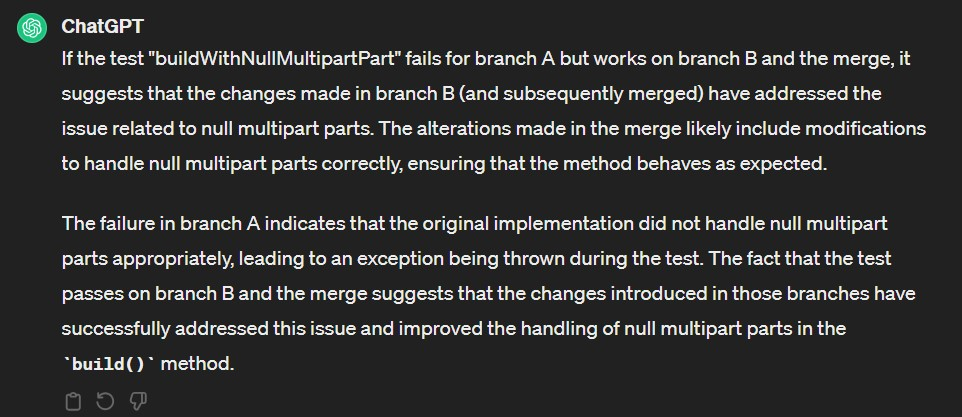
\includegraphics[width=1\linewidth]{figures/testexplain.jpg}
    \caption{ChatGPT explanation of meaning of failures and passes of test in different branches}
    \label{fig:testexplain}
\end{figure}

Common issues affecting test generation were:

\begin{itemize}
  \item Faulty importing/setup: Particularly relevant in the OKHttp case, the tool was patently unable to correctly call imports, just omitting them, even when expressly being given the package names and being told to import it.
  \item Invalid access: The LLM was generally unable to distinguish between private and public methods and frequently made attempts to invoke or access private methods and fields.
  \item Method/Field/Class Hallucination: ChatGPT frequently invoked non-existent methods, fields or even classes. In some classes this could also be related to matters of access, as it generated getter calls for private fields.
  \item Incomplete/Template Tests: Despite being prompted explicitly to generate complete tests that should compile, in several cases tests were generated with incomplete template helper methods and classes.
\end{itemize}

While feeding compilation error outputs could be a solution for these, in practice no test that failed to compile was fixed in this manner, as changes made did not fix or ignored the problems present. In some cases, while the logic of correction was sound logically, they were not helpful in the context of automatic test generation. For example, a "MockConverter" class was used in a test for the Retrofit project. Upon prompting for a fix, an import was added, which still naturally was non-functional. Upon prompting for another fix, ChatGPT provided a basic empty template for the MockConverter class. While a correctly implemented MockConverter class would fix the issue and allow the test to compile, the solution here would have been to drop the usage of the MockConverter class in the first place

Experiments were made to employ the usage of vector indexing to boost the capabilities of understanding code. The theory was that, by indexing the entire repository of code, we could proceed with prompting without having to decide which specific blocks of code should be required information in the prompt and that, during generation, the LLM could correctly identify the chain of dependencies, and which methods and parameters should be employed to properly test our desired methods. In this process we employed llama\_index, but the results fell short: due to an observed worse ability to generating code, focus was placed on the explanation of what should be done, with the prompting: "We want to create an extensive testing suite for the method [method] of the class [class]. How should we approach this? Which calls should we make, which parameters should we try and which results should be expected?"
Results were generic, many times not even referring to aspects of the code itself and still prone issues of hallucination, specifically the making of references to non-existent methods.

\section{Comparison of Developed Prompts with State of the Art}

To evaluated our progressively developed prompt with existing state of the art, we selected 5 prompts from comparison, henceforth referred as 1 \cite{kn:chattester}, 2 \cite{kn:siddiq2023empirical}, 3 \cite{kn:gptunitbra} and 4 \cite{kn:chatunitest}. Our prompt, in turn, was 2-step prompt as follows:

\begin{quote}
The following class was altered in a merge, specifically the METHOD method. Analyse it and what it does, with focus on the method and its usage: CLASS INFO
\end{quote}

\begin{quote}
You are a Java developer. Due to changes in the METHOD method, you've been asked to write a complete test suite to identify possible errors introduced due to the changes. Write a junit test suite for the method. All classes must be correctly imported. The tests must compile without errors. The tests must be complete and require no modification and addition. No explanation needed.
\end{quote}

As subjects, we selected the basic fabricated Point class example, Antlr4, whose testing simply requires the length of a returned list and OkHttp, a more complex example requiring mocks and reflection for testing.
For each prompt, we generated 3 times and selected the best result for comparison.

For Point, we made the following observations:

Our prompt generated a suite with 3 tests, one of which had an incorrect assertion (A Point with coordinates -3,-4 was expected to move to 4,5 when it should move to 4,3). Despite this one wrong test, the correct ones successfully identified the conflict, as they tested manhattan distance movement. For an earlier branch, with euclidian distance movement, they would fail, showing the conflict.

Prompt 1 called the distance() method to identify where the Point should be and set assertions accordingly. While this tested the move method, it could not identify the conflict, as the assertions were dependent on the behaviour of distance(), as it changed so did they.

Prompt's 2,3,4 all made the same mistake: Starting from a point 3,4, they expected it to move to 7,8. As distance is 7, it should actually move to 10,11. Notably, Prompt 3 and 4 generated tests for distance and correctly identified it as 7.

For Antlr4, our prompt ran into errors: it could not correctly initialize the class, as the CodeGenerator object called by the constructor was incorrectly created. It also severely undercounted the number of keywords, leading to an incorrect assertion.
Prompt 1 showed improvement over ours, as it understood a null could be used in place of CodeGenerator, as it would not be used for our purposes. Despite this, it failed in the logic of the test, calling badWords unnecessarily: this is a private method that is already called by the getBadWords method we are testing. This same error was present in Prompt 2.
Prompt 3 generated nonsensical tests, just checking if the result of methods called was false. While it tested non-existent methods, it did not tested getBadWords as we desired.
Prompt 4 also called addBadWords despite not needing it, but as it was instructed to use Mockito, it avoided the error of calling a private method by using reflection. The rest of the test logic and the assertion was correct.


OkHttp should be the hardest to test, as the method under test and the method which calls it are private. The value returned (which we seek to test) is never publicly available.
Thus all prompts try and fail to call the private method. The exception is Prompt 3 which, by it's nature of generating for all methods rather than being told to generate for a specific one, avoids private methods. Surprisingly, Prompt 4 which had shown ability to use reflection in the previous subject, failed to produce a satisfactory result. Also of note is Prompt 2, which calls for 10 tests to be generated: in this case, to reach this 'quota', each parameter of the copied client was tested in a entirely different test, rather than just in a different assertion.
Despite failing, due to previously mentioned issue with access, Prompt 1 notably produced the best assertions, as it tested both functionalities of the method: the correct copying of defined parameters, and the returning of defaults for parameters that were not set.

\section{Research Question 1}

The first research question we established sought to more systematically evaluate ChatGPT's capabilities to assess and describe semantic conflicts: "Can ChatGPT identify, understand and explain whether there is a semantic conflict in a merge commit?"
To evaluate this research question, we established 8 subjects:
3 fabricated scenarios, one on a Point class and 2 by Nuno Castanho \cite{kn:nuno}, that had shown success in earlier experiments.
3 fabricated scenarios on a Cart class. These represent conflicts of type Parallel Changes in Field, Parallel Changes in Method and Change Method, which were shown to be the most common in real world scenarios \cite{kn:nuno}. Finally, 2 real world scenarios, in the Antlr and OkHttp projects.


For assessment, we established 5 metrics, with likert scales:

-A: Changes between branches correctly identified (Correct description of Version A and B)

0: Large errors in description for both branches

1: Large error in description of one branch

2: Minor insignificant errors

3: Changes correctly identified

-B: No conflict misunderstanding (Does not describe textual conflict, understand merge succeed)

0: Understands conflict as textual

1: Understands the conflict as semantic

-C: Positive response (3 types: says conflict exists/may exist/does not exist)

0: Denies existence of conflict

1: Asserts conflict is possible

2: Asserts conflict exists

-D: Origin of conflict described (What code interactions lead to altered behaviour)

0: Incorrect or non-existent explanation

1: Identifies origin of conflict, with lack of clarity or imprecisions

2: Identifies origin of conflict, with lack of confidence

3: Identifies origin of conflict

-E: Effect of conflict described (What is the result of the code interactions/expected output)

0: Result of conflict is omitted, too vague or wrong

1: Result of conflict is expressed, but with imprecisions or generically

2: Possible code outputs are expressed, with little confidence

3: Assertively points out expected outputs due to conflict

For the purposes of this research question, we settled on a final prompt:

\begin{quote}
You are a software developer that has to assess whether there is a semantic conflict in a merge commit.  Given the base version of the class, the diff from base to a version A, the diff from base to a version B and the merged version of the class, assess whether there is a semantic conflict and explain it.

Base version:
```java
```

Diff version A and the base:
```diff
```

Diff version B and the base:
```diff
```

Merge version:
```java
```

\end{quote}

For each semantic conflict example, the prompt would be submitted 3 times, allowing us to see a broader range of responses and avoiding what might be one-time flukes.

The complete prompts, with results and evaluated metrics, can be found in the attachments. The following is just the results, with metric evaluations and necessary comments.

\subsection{Point}

Answer 1 was:
\begin{lstlisting}
Based on the provided information, let's analyze the changes in versions A and B and then compare them with the merged version to assess whether there is a semantic conflict.

Version A introduces a change in the `move()` method:
```java
-         this.x += 1;
-         this.y += 1;
+         double dist = distance();
+         this.x += dist;
+         this.y += dist;
```
This change calculates the distance from the origin to the point and moves the point by that distance in both x and y directions.

Version B modifies the `distance()` method:
```java
-        return Math.sqrt(Math.pow(getX(), 2)+ Math.pow(getY(), 2));
+        return Math.abs(getX())+Math.abs(getY());
```
This change alters the calculation of the distance between the point and the origin to simply summing the absolute values of x and y coordinates.

Now, let's compare these changes with the merged version:
```java
public class Point {
    private double x;
    private double y;

    public Point(double x, double y) {
        this.x = x;
        this.y = y;
    }

    public double getX() {
        return x;
    }

    public double getY() {
        return y;
    }

     public void move() {
         double dist = distance();
         this.x += dist;
         this.y += dist;
     }

    public double distance() {
        return Math.abs(getX())+Math.abs(getY());
    }

    public String toString() {
        return "(" + getX() + ", " + getY() + ")";
    }
}
```
In the merged version, the `move()` method is modified to match the changes introduced in version A, and the `distance()` method is also updated to match the changes introduced in version B.

Considering the changes made in both versions A and B are applied consistently in the merged version without introducing any conflicts or contradictions, there doesn't seem to be a semantic conflict in this merge commit. The modifications from both branches are complementary and do not interfere with each other's functionality. Therefore, the merge appears to be successful in integrating the changes from both branches.
\end{lstlisting}

With metrics:
A:3
B:1
C:0
D:0
E:0



Answer 2 was:
\begin{lstlisting}
To assess whether there is a semantic conflict in the merge commit, let's analyze the changes introduced in versions A and B compared to the base version, and then compare them with the merged version.

### Changes introduced in Version A:
- The `move()` method has been modified to calculate the distance using the `distance()` method and then update the `x` and `y` coordinates accordingly.
- This change effectively moves the point by the distance it currently is from the origin.

### Changes introduced in Version B:
- The `distance()` method has been modified to calculate the Manhattan distance instead of the Euclidean distance.
- The Manhattan distance is calculated by taking the absolute value of the x and y differences.

### Analysis of Merged Version:
- The `move()` method from Version A has been kept in the merged version, which calculates the distance using the Euclidean distance.
- The `distance()` method from Version B has been kept, which calculates the Manhattan distance.

### Potential Semantic Conflict:
- The potential conflict arises from the inconsistency between how distance is calculated in the `move()` method and the `distance()` method in the merged version.
- While the `move()` method assumes Euclidean distance for movement, the `distance()` method calculates the Manhattan distance.
- This inconsistency could lead to unexpected behavior, as the `move()` method might not accurately reflect the intended behavior of the `distance()` method.

### Conclusion:
- There is a semantic conflict in the merge commit because the merged version contains methods with conflicting assumptions about how distance should be calculated.
- Resolving this conflict would require ensuring consistency in the distance calculation method used throughout the class, either sticking with Euclidean distance or Manhattan distance for both `move()` and `distance()` methods.
\end{lstlisting}

With metrics:
A:3
B:1
C:2
D:3
E:2

Answer 3 was:
\begin{lstlisting}
To assess whether there is a semantic conflict in the merged version of the `Point` class, let's compare the changes introduced in versions A and B and then examine the resulting merged version.

Version A introduced a change in the `move()` method, where instead of incrementing both `x` and `y` coordinates by 1, it calculates the distance from the origin using the `distance()` method and increments both coordinates by this distance.

Version B modified the `distance()` method to calculate the distance using the absolute values of `x` and `y` coordinates instead of using the Euclidean distance formula.

Now, let's analyze the merged version:

- The `Point` class constructor, `getX()`, `getY()`, and `toString()` methods remain unchanged from the base version, as there were no conflicting modifications in these areas.
- The `distance()` method in the merged version matches the changes introduced in version B, using the absolute values of `x` and `y` coordinates.
- The `move()` method in the merged version also matches the changes introduced in version A, calculating the distance using the modified `distance()` method and updating both `x` and `y` coordinates accordingly.

Considering these changes, there doesn't seem to be a semantic conflict in the merged version. Both changes from versions A and B are compatible, and they integrate seamlessly without introducing contradictions or inconsistencies. Therefore, the merged version appears to be correct in terms of maintaining the intended functionality of the `Point` class. 
\end{lstlisting}

With metrics:
A:3
B:1
C:0
D:0
E:0

This first example shows particularly the importance of running several trials as despite the simplicity of the conflict, the LLM fails to identify it 2/3 times. Despite this, when it does identify it, it puts forth a good description.

\subsection{Fabricated, Remove Override}

Answer 1 was:
\begin{lstlisting}
Based on the provided information, let's analyze the changes made in versions A and B, and then compare them with the merge version to assess if there is a semantic conflict.

In version A, the following changes were made:
1. Added a method `hashString()` which computes the hash code of the string representation returned by the `helpString()` method.

In version B, the following changes were made:
1. Removed the `helpString()` method.

Now, let's look at the merge version:
- It retains the addition of the `hashString()` method from version A.
- It removes the `helpString()` method as done in version B.

There is a semantic conflict between the changes made in versions A and B:
- Version A adds the `hashString()` method that relies on the `helpString()` method.
- Version B removes the `helpString()` method which is used by `hashString()`.

This results in a semantic conflict because the `hashString()` method in the merge version depends on the `helpString()` method which has been removed in version B. Therefore, if the `hashString()` method is invoked in the merge version, it will cause an error because the `helpString()` method is no longer available.

To resolve this conflict, you may need to decide whether to keep the `hashString()` method and reintroduce the `helpString()` method or remove the `hashString()` method altogether, depending on the intended functionality of the merged class.
\end{lstlisting}

With metrics:
A:3
B:1
C:2
D:3
E:1

Answer 2 was:
\begin{lstlisting}
Based on the provided information, let's analyze the changes introduced in versions A and B, and then examine the merged version to determine if there's a semantic conflict.

In version A, the following method was added:
```java
public int hashString(){
    return helpString().hashCode();
}
```

In version B, the following method was removed:
```java
public String helpString(){
    StringBuilder result = new StringBuilder();
    result.append(super.toString());
    if(lugares != null)
        result.append(" | Lugares: " + lugares.size());
    else
        result.append(" | Lugares: null");
    return result.toString();
}
```

The merged version includes the method `hashString()` from version A and does not include the method `helpString()` from version B.

Now, let's analyze the potential conflict:

1. **Method Addition (from version A):** Adding `hashString()` doesn't conflict semantically with the base version or version B since it's a new method.

2. **Method Removal (from version B):** Removing `helpString()` could potentially cause a conflict if any code in the project relied on this method. However, since `helpString()` doesn't seem to be essential for the functionality provided in the class, its removal may not cause any immediate semantic issues.

In conclusion, there doesn't seem to be a significant semantic conflict in this merge. The changes in both versions A and B are related to methods that don't directly affect the core functionality of the class. Therefore, the merge appears to be valid. However, it's always a good practice to verify the impact of method removals, especially if they are being used elsewhere in the codebase.
\end{lstlisting}

With metrics:
A:3
B:1
C:0
D:0
E:0

Answer 3 was:
\begin{lstlisting}
Based on the provided information, let's analyze the changes introduced in versions A and B, and then compare them with the merged version to identify any potential semantic conflicts.

In version A, the following method was added:
```java
public int hashString(){
    return helpString().hashCode();
}
```

In version B, the following method was removed:
```java
public String helpString(){
    StringBuilder result = new StringBuilder();
    result.append(super.toString());
    if(lugares != null)
        result.append(" | Lugares: " + lugares.size());
    else
        result.append(" | Lugares: null");
    return result.toString();
}
```

Now, let's look at the merged version. In the merged version, the `hashString()` method from version A was retained, but the `helpString()` method from version B was removed.

There is a potential semantic conflict here because the `hashString()` method in version A relies on the `helpString()` method, which was removed in version B. Therefore, calling `hashString()` in the merged version will result in a compilation error or unexpected behavior since the `helpString()` method is not present anymore.

To resolve this conflict, you would need to either reintroduce the `helpString()` method in the merged version or remove the `hashString()` method, depending on the intended functionality of the class. If `hashString()` is necessary, you would need to reimplement it without relying on `helpString()` or ensure that `helpString()` is also present in the merged version.
\end{lstlisting}

With metrics:
A:3
B:1
C:1
D:3
E:1

\subsection{Fabricated, Overload by Access Change}

Answer 1 was:
\begin{lstlisting}
In the provided scenario, let's analyze the merge commit and determine if there are any semantic conflicts.

The merge commit introduces a new method in the `Event` class:

```java
public int setProducerNumber(int n){
    if(producer != null){
        producer.setResgistrationNumber(n);
        return producer.getRegistrationNumber();
    }
    return -1;
}
```

This method seems to be intended to set the registration number of the producer associated with the event. However, there's a potential issue with this method name and its intended functionality:

1. **Method Name Conflict**:
   - In version A, the method `setResgistrationNumber(int resgistrationNumber)` is added to the `Producer` class.
   - In version B, the method `setProducerNumber(int n)` is added to the `Event` class.

These methods have similar names but operate on different classes. The method `setResgistrationNumber` in the `Producer` class seems to be intended for setting the registration number of a producer. However, the method `setProducerNumber` in the `Event` class seems to be intended to set the registration number of the producer associated with the event. There's a spelling mistake in both method names, but this doesn't directly affect the semantic conflict. The real issue lies in the ambiguity of the method names and their purposes.

2. **Encapsulation Violation**:
   - The method `setResgistrationNumber(int resgistrationNumber)` in the `Producer` class is changed from public to private in version A, which implies a change in its accessibility.
   - However, the method `setProducerNumber(int n)` in the `Event` class is intended to set the registration number of the producer, implying that it should be accessible from outside the class. Making the corresponding method in the `Producer` class private conflicts with this intention, potentially preventing the intended functionality.

3. **Semantic Clarity**:
   - There's a need for clarity regarding which class should be responsible for setting the registration number of the producer associated with an event. Is it the `Producer` class itself or the `Event` class? This should be clarified for proper code organization and maintainability.

To resolve this conflict, you need to clarify the responsibilities of each class and ensure that method names are clear and unambiguous. It might involve renaming methods, revisiting encapsulation decisions, and ensuring that the functionality aligns with the intended design of the system.
\end{lstlisting}

With metrics:
A:1
B:1
C:0
D:3
E:1

Answer 2 was:
\begin{lstlisting}
In the provided scenario, let's analyze the changes made in versions A and B and then see if there's a semantic conflict in the merge commit.

### Version A Changes:
1. The method `setResgistrationNumber(int resgistrationNumber)` in the `Producer` class was changed to `private`.

### Version B Changes:
1. A new method `setProducerNumber(int n)` was added to the `Event` class, which sets the registration number of the producer.
   - This method internally calls `producer.setResgistrationNumber(n)`.

### Merge Commit:
The merge commit contains changes from both versions A and B. It includes the changes in the `Producer` class from version A and the changes in the `Event` class from version B.

### Semantic Conflict Assessment:
1. The change in version A made `setResgistrationNumber(int resgistrationNumber)` private in the `Producer` class.
2. The change in version B introduced a new method `setProducerNumber(int n)` in the `Event` class, which attempts to set the registration number of the producer.
   - This new method internally tries to access `producer.setResgistrationNumber(n)`, which is now private due to the change in version A.

### Conclusion:
There is a semantic conflict in the merge commit. The conflict arises because the `setProducerNumber(int n)` method in the `Event` class tries to access a method (`setResgistrationNumber(int resgistrationNumber)`) in the `Producer` class that has been made private in version A. As a result, this merge may lead to compilation errors or unexpected behavior in the application, as the method access is not allowed due to its visibility being changed to private. To resolve this conflict, you may need to modify either the visibility of the method in the `Producer` class or refactor the code in the `Event` class to not rely on this method directly.
\end{lstlisting}

With metrics:
A:3
B:1
C:2
D:3
E:1

Answer 3 was:
\begin{lstlisting}
To assess whether there is a semantic conflict in the merge commit, we need to analyze the changes introduced in versions A and B separately and then examine the merged version for any potential conflicts. Let's break down the changes:

### Diff A (Version A changes):
1. Changed the visibility of the method `setResgistrationNumber(int resgistrationNumber)` in the `Producer` class from public to private.

### Diff B (Version B changes):
1. Added a new method `setProducerNumber(int n)` in the `Event` class, which sets the registration number of the associated `Producer` if it exists.

### Merge Version:
The merge version includes both changes from versions A and B, along with the base version.

Now, let's analyze the potential conflicts:

1. **Method Visibility Conflict:**
   - Version A changes the visibility of `setResgistrationNumber` in the `Producer` class to private, while version B introduces a new method `setProducerNumber` in the `Event` class, which attempts to call `producer.setResgistrationNumber(n)`.
   - Since `setResgistrationNumber` is now private, it cannot be accessed from outside the `Producer` class, leading to a semantic conflict. The attempt to call this method in `setProducerNumber` will result in a compilation error.

### Conclusion:
The semantic conflict arises due to the attempt to access a private method (`setResgistrationNumber`) from another class (`Event`) in the merged version. This conflict needs to be resolved by either making `setResgistrationNumber` accessible (e.g., changing its visibility back to public), modifying the way registration number is set, or restructuring the code to avoid this dependency altogether.
\end{lstlisting}

With metrics:
A:3
B:1
C:1
D:3
E:0

In these fabricated examples, the biggest issue remained the identification of the effects of the semantic conflict, namely that when an overriden function was removed or had its' access changed, the other function, with different behaviour, would be used instead. However, given the constraints of the prompt, which is limited to one class, the necessary information could not be transmitted and the LLM argued there would be compilation errors. Better results were observed when doing more manual, ad-hoc experiments, as we could identify exactly all the classes involved in the conflict and offer all the required information.

\subsection{Cart, Change Method}

Answer 1 was:
\begin{lstlisting}
Based on the provided code snippets, let's analyze the changes and the merged version:

1. **Diff A (version A vs. base)**:
   - It introduces a conditional check inside the `total_cost` method to handle the case where `user.admin` is true, returning 0 in that case.

2. **Diff B (version B vs. base)**:
   - It introduces a conditional check inside the `checkout` method to ensure that the `cost` calculated is not equal to 0; otherwise, it throws a `RuntimeException`.

3. **Merge version**:
   - It combines the changes from both versions A and B with the base version.

Now, let's assess for potential semantic conflicts:

- The addition of the `if(user.admin)` check in version A doesn't directly conflict with the change in version B where it checks for `cost == 0`. These changes seem to be orthogonal, addressing different concerns (user privileges vs. checkout validation).
  
- However, there is a potential semantic conflict between the `total_cost` method in version A and the `checkout` method in version B. If `user.admin` is true, `total_cost` will return 0, potentially causing the `checkout` method in version B to throw a `RuntimeException` even if `user.admin` is true, which might not be intended.

To resolve this conflict, consider adjusting the conditions or the logic to ensure consistency between the `total_cost` and `checkout` methods when dealing with the scenario of an admin user.

Overall, there is a potential semantic conflict that needs to be addressed to ensure the correct behavior of the merged version.
\end{lstlisting}

With metrics:
A:3
B:1
C:1
D:2
E:2

Answer 2 was:
\begin{lstlisting}
Based on the provided information, let's analyze the merge commit and identify any potential semantic conflicts:

1. **Diff A and Base:**
   - Introduces a condition in the `total_cost` method, returning 0 if the user is an admin.
   - This change ensures that if the user is an admin, the cost will always be zero.

2. **Diff B and Base:**
   - Introduces a condition in the `checkout` method, throwing an exception if the cost is 0.
   - This change ensures that if the cost is calculated to be 0, an exception is thrown, preventing checkout with a 0 cost.

3. **Merged Version:**
   - Incorporates both changes from Diff A and Diff B.
   - The `total_cost` method checks if the user is an admin and returns 0 accordingly.
   - The `checkout` method checks if the cost is 0 and throws an exception if so.

There doesn't seem to be a direct semantic conflict between the changes from versions A and B. However, there might be a potential issue related to the logic flow. If the user is an admin and a discount code that results in a cost of 0 is applied, the exception will never be thrown because the `checkout` method won't be called. This scenario might need to be considered depending on the desired behavior.

In summary, while there is no direct conflict between the changes, the merged version should be reviewed to ensure that the logic flow is consistent with the desired behavior. Depending on the requirements, adjustments might be needed to handle cases where an admin applies a discount resulting in a cost of 0.
\end{lstlisting}

With metrics:
A:3
B:1
C:0
D:0
E:0

Answer 3 was:
\begin{lstlisting}
In the merged version of the `Cart` class, let's analyze the changes and their potential implications:

1. **Changes from Version A (Base to A):**
   - Added a condition in the `total_cost` method: `if(user.admin) return 0;`
   - This implies that if the user is an admin, the total cost of the cart will always be zero.

2. **Changes from Version B (Base to B):**
   - Added a condition in the `checkout` method: `if(cost==0) throw new RuntimeException("Cost can't be 0");`
   - This implies that if the calculated cost of the cart is zero, it throws a `RuntimeException`.

3. **Merged Version (Merged A and B with Base):**
   - Both changes from versions A and B are present in the merged version.

Now, let's consider how these changes interact:

- In the merged version, the `total_cost` method from Version A sets the cost to zero if the user is an admin.
- However, in the `checkout` method from Version B, if the cost is zero, it throws an exception, indicating that a zero cost is not acceptable.

This is a semantic conflict because:

- Version A assumes that setting the cost to zero for an admin is acceptable behavior.
- Version B assumes that a zero cost is not acceptable and throws an exception if encountered during checkout.

This conflict arises from the different assumptions and behaviors of the two versions regarding the handling of zero costs. As a result, it may lead to unexpected behavior or exceptions during execution, especially if the admin status of a user is incorrectly handled or if the conditions for zero cost calculation are not properly synchronized between the methods.
\end{lstlisting}

With metrics:
A:3
B:1
C:2
D:3
E:0

We see variability in these results. Notably, in the cases where the conflict is identified, with varying exactness, it falls short of being able to explain the exact result of the conflict, namely that if an admin tries to checkout, there will always be a exception thrown.

\subsection{Cart, Parallel Field}

Answer 1 was:
\begin{lstlisting}
In the merged version, there is a semantic conflict in the `discounts` map initialization due to conflicting changes introduced in both versions A and B.

Let's break it down:

- Version A adds a new discount code "megasaver" with a discount of 0.4.
- Version B modifies the discount of the "superpromo" code to 0.25.

During the merge, both changes are attempted to be integrated into the base version.

The conflict arises because both Version A and Version B attempt to modify the same line in the `discounts` map initialization. However, they are modifying different entries within that line.

Here's the relevant portion of the merged version:

```java
private static final Map discounts = Collections.unmodifiableMap(new HashMap<>() {{
    put("loyal", 0.1d);
    put("megasaver", 0.25d); // Conflicting change from version B
    put("30ff", 0.3d);
    put("2024", 0.2d);
    put("megasaver", 0.4d); // Conflicting change from version A
}});
```

As you can see, both Version A and Version B are trying to set the discount for "megasaver" code, but to different values (0.4d in Version A and 0.25d in Version B). This creates a semantic conflict because the merge cannot automatically determine which value to use for the "megasaver" discount.

To resolve this conflict, a developer would need to manually intervene and decide which discount value to keep for the "megasaver" code, or possibly merge both changes if they are compatible in some way.
\end{lstlisting}

With metrics:
A:1
B:1
C:2
D:1
E:0

Answer 2 was:
\begin{lstlisting}
In this scenario, let's analyze the changes introduced by each version:

1. **Version A**:
   - It adds a new discount code `"megasaver"` with a discount of 0.4d.

2. **Version B**:
   - It changes the discount value for the `"superpromo"` code from 0.25d to 0.25d.

Now, let's look at the merge commit:

- In the merge version, the `"megasaver"` discount code is listed twice in the map, once with a value of 0.25d and once with a value of 0.4d.

This constitutes a semantic conflict. The conflict arises because both versions A and B try to modify the `"megasaver"` discount, but they assign different values to it. In the merge commit, the conflict resolution results in keeping both changes, resulting in duplicate entries for the `"megasaver"` discount code with different values. This could lead to unintended behavior when applying discounts during checkout, as the system might use one of the conflicting values or encounter unexpected behavior due to duplicate keys.

To resolve this conflict, you would need to manually choose which value for the `"megasaver"` discount should be kept or find an appropriate compromise that preserves the intended behavior of the class.
\end{lstlisting}

With metrics:
A:1
B:1
C:2
D:3
E:1

Answer 3 was:
\begin{lstlisting}
In the provided scenario, there is indeed a semantic conflict in the merge commit. Let's break down the changes from versions A, B, and the merge to understand the conflict:

- Version A introduces a new discount code called "megasaver" with a discount value of 0.4.
- Version B modifies the discount value of the "superpromo" code to 0.25 instead of 0.3.

Now, let's analyze the merge commit:

- In the merge commit, both changes from versions A and B are included, resulting in the following discount map:
```java
private static final Map discounts = Collections.unmodifiableMap(new HashMap<>() {{
    put("loyal", 0.1d);
    put("megasaver", 0.25d); // Conflict here!
    put("30ff", 0.3d);
    put("2024", 0.2d);
    put("megasaver", 0.4d); // Conflict here!
}});
```

The conflict arises because both version A and version B attempt to modify the same key in the discounts map, "megasaver", with conflicting values (0.25 and 0.4, respectively). This means that after the merge, the final discount for "megasaver" will depend on the order of the changes applied, which can lead to unexpected behavior.

To resolve this semantic conflict, you need to decide which discount value should be used for the "megasaver" code or whether both should be kept with different keys. Additionally, you may need to communicate with your team to ensure consistency and prevent future conflicts.
\end{lstlisting}

With metrics:
A:1
B:1
C:2
D:3
E:1

In this case, ChatGPT consistently failed to accurately describe the changes made, however this did not worsen it's ability to identify the conflict. However it also consistently falls back on vaguer descriptions on the result: in an ideal scenario we would hope it would be able to point out that the 0.4d value, set last, would override 0.25d.

\subsection{Cart, Parallel Method}

Answer 1 was:
\begin{lstlisting}
Based on the provided information, let's analyze the changes made in versions A and B relative to the base version, as well as the resulting merge version.

1. **Change in Version A**:
   - In the `sum_items()` method, the line `return Math.max(0, sum);` was modified to `return sum;`.
   - This change removes the condition that ensures the sum is at least 0 before returning it.

2. **Change in Version B**:
   - In the `sum_items()` method, a conditional statement was added:
     ```java
     if(item.coupon)
         sum -= item.value*item.amount;
     else
         sum += item.value*item.amount;
     ```
   - This change adjusts the sum calculation based on whether an item has a coupon.

Now, let's consider the merge version:

- The merge version incorporates both changes from versions A and B.

In the merge version:
- The `sum_items()` method is adjusted to include the conditional statement from Version B, but it doesn't have the Math.max() check from Version A.

### Potential Semantic Conflict:
- The semantic conflict arises due to the difference in behavior of the `sum_items()` method between Version A and Version B.
- Version A returns the maximum of 0 and the sum, ensuring that the total sum is non-negative.
- Version B modifies the sum calculation based on whether an item has a coupon, potentially resulting in a negative sum if there are items with coupons that reduce the total.

### Explanation:
- If there are items with coupons that reduce the total (which is the case in Version B), the absence of the Math.max() check in the merge version (which was present in Version A) can lead to a semantic conflict.
- Without the Math.max() check, the merge version may produce a negative sum if the total discounts exceed the total item costs, which could lead to incorrect calculations or unexpected behavior during checkout or other operations involving the cart.

### Resolution:
- To resolve this conflict, the merged version should retain the Math.max() check from Version A or incorporate a similar check to ensure that the sum returned by `sum_items()` is non-negative, aligning with the behavior intended by the base version.
\end{lstlisting}

With metrics:
A:3
B:1
C:1
D:3
E:3

Answer 2 was:
\begin{lstlisting}
Based on the provided information, let's analyze the changes made in versions A and B compared to the base version, and then compare them with the merged version.

Version A introduces a change in the `sum_items()` method, removing the `Math.max(0, sum)` line and returning `sum` directly.

Version B introduces a conditional statement within the `sum_items()` method, where if `item.coupon` is true, it subtracts `item.value * item.amount` from the sum; otherwise, it adds `item.value * item.amount` to the sum.

Now, let's look at the merged version:

```java
public double sum_items() {
    double sum = 0;
    for(Item item: cartItems) {
        if(item.coupon)
            sum -= item.value*item.amount;
        else
            sum += item.value*item.amount;
    }
    return sum;
}
```

In the merged version, it combines the changes from both versions A and B. It retains the conditional statement introduced in version B, making the sum calculation conditional based on the `item.coupon` value.

There doesn't seem to be a direct semantic conflict between the changes introduced in versions A and B. Both versions modify the `sum_items()` method to adjust the sum calculation logic, but they are compatible changes.

In version A, the change made might be seen as simplifying the logic, removing the unnecessary `Math.max(0, sum)` line, while version B introduces a more complex logic with the conditional statement, probably to handle special cases related to coupons. The merged version appropriately combines these changes without conflicts.

Therefore, there is no semantic conflict in the merged version.
\end{lstlisting}

With metrics:
A:3
B:1
C:0
D:0
E:0

Answer 3 was:
\begin{lstlisting}
From the provided base version and the diffs, let's analyze the changes:

1. **Diff version A**:
   - Changes the `sum_items()` method to remove the `Math.max(0, sum)` operation and returns the raw sum.
   
2. **Diff version B**:
   - Modifies the `sum_items()` method to handle a new scenario where if an item has a coupon, it subtracts its value from the sum instead of adding it.
   
Now, let's examine the merged version:

- The merged `sum_items()` method combines changes from both versions A and B, resulting in logic that adds or subtracts item values based on whether a coupon is present.
  
There isn't a direct conflict between the changes in versions A and B because they modify different aspects of the `sum_items()` method. However, there is a potential semantic conflict depending on the intended behavior of the system:

- Version A removes the restriction that the sum of items should be non-negative.
- Version B introduces a new scenario where item values are subtracted from the sum based on the presence of a coupon.

The conflict arises if it's not intended for the sum of items to become negative, which is a possibility in the merged version due to the removal of `Math.max(0, sum)` and the introduction of coupon handling. If the system's requirements mandate that the sum of items should always be non-negative, then this would be a semantic conflict, as the merged version does not enforce that restriction.

In summary, while there isn't a direct conflict between the changes in versions A and B, there is a potential semantic conflict introduced in the merged version regarding the non-negativity of the sum of items, depending on the system's requirements.
\end{lstlisting}

With metrics:
A:3
B:1
C:1
D:3
E:3

Despite one failure of detection, this example provided very good results, both in identifying and describing the consequences of the conflict.

\subsection{Antlr}

Answer 1 was:
\begin{lstlisting}
In order to assess whether there's a semantic conflict in the merge commit, let's analyze the changes introduced in versions A and B compared to the base version, and then inspect the merged version.

1. **Diff A vs Base:**
   - In version A, the `reduce` keyword was replaced with `return` in the `python2Keywords` array.

2. **Diff B vs Base:**
   - In version B, the `del` keyword was added to the `python2Keywords` array.

3. **Merged Version:**
   - The merged version includes both changes from versions A and B.

Now, let's consider the semantic implications:

- **Version A** replaces `reduce` with `return`. This change seems reasonable as `return` is a keyword used in functions to return values whereas `reduce` is a function for applying a function to all elements of an iterable.
  
- **Version B** adds the `del` keyword. This is also sensible as `del` is used to delete objects.

- **Merged Version** includes both changes, incorporating `return` from Version A and `del` from Version B.

Upon examining the merged version, it appears there is no direct semantic conflict. Both changes are additions or replacements of Python keywords, and they don't interfere with each other. The `return` keyword addition and the `del` keyword addition are unrelated in terms of their functionality within Python.

Thus, based on the provided information, there doesn't seem to be a semantic conflict in the merge commit. However, it's essential to perform thorough testing to ensure the correctness and compatibility of the merged code with the intended functionality.
\end{lstlisting}

With metrics:
A:1
B:1
C:0
D:0
E:0

Answer 2 was:
\begin{lstlisting}
In order to assess whether there's a semantic conflict in the merge commit, let's analyze the changes introduced in versions A and B and compare them with the merged version.

Version A introduces the change:
```diff
                "range", "raw_input", "reduce", "reload", "repr", "return", "reversed", "round",
```

Version B introduces the change:
```diff
                "del", "delattr", "dict", "dir", "divmod",
```

Both versions introduce modifications to the list of reserved keywords in the `Python2Target` class.

Now let's look at the merged version. It includes changes from both version A and version B:
```java
		"del", "delattr", "dict", "dir", "divmod",
		"range", "raw_input", "reduce", "reload", "repr", "return", "reversed", "round",
```

From the merged version, it appears that both changes were integrated successfully without any conflicts. The merged version contains all keywords from both versions A and B.

However, one notable change is the addition of the keyword `"del"` from version B, which was not present in version A. This change might be considered risky, as "del" is a commonly used keyword in Python for deleting variables, items, or slices. Its inclusion in the reserved keywords list might lead to unintended behavior if the code attempts to use "del" as an identifier elsewhere.

Therefore, while there is no direct semantic conflict, the inclusion of the "del" keyword should be carefully reviewed to ensure it doesn't inadvertently affect the behavior of the code that uses instances of `Python2Target`. It would be advisable to review the usage of this keyword within the context of the class and its potential impact on existing or future code using instances of this class.  
\end{lstlisting}

With metrics:
A:3
B:1
C:0
D:0
E:0

Answer 3 was:
\begin{lstlisting}
Based on the provided information, let's analyze the merge commit and check for any semantic conflicts:

1. **Diff A vs. Base**:
   - Addition of `"return"` keyword in the `python2Keywords` array.
   - No conflicting changes with other methods or properties.

2. **Diff B vs. Base**:
   - Replacement of `"delattr"` with `"del"` in the `python2Keywords` array.
   - No conflicting changes with other methods or properties.

3. **Merge Version**:
   - Both changes from Diff A and Diff B are present in the merge version.
   - `"return"` and `"del"` keywords are both added to the `python2Keywords` array.

There doesn't seem to be a semantic conflict between the changes introduced in the merge commit. Each change from the parent branches (A and B) applies cleanly without interfering with each other. The merge version includes both additions (`"return"` and `"del"`) without causing any inconsistencies or clashes.

Hence, from a semantic perspective, the merge seems successful without any conflicts. Each change integrates cleanly with the base version, resulting in a coherent final version.
\end{lstlisting}

With metrics:
A:1
B:1
C:0
D:0
E:0

No conflict was identified. Notably there was also repeated failure in describing the changes made on the branches. We observed this before with the Parallel Field example in cart, so it is possible the fact that the changes are being made to fields may have some relation.

\subsection{OkHttp}

Answer 1 was:
\begin{lstlisting}
To assess whether there is a semantic conflict in the merge commit, let's analyze the changes introduced in versions A and B separately and then compare them in the merged version.

### Changes in Version A:
1. Added import statement: `import com.squareup.okhttp.internal.Util;`.
2. Added field `private List<String> transports`.
3. Modified the constructor to initialize `transports` and `failedRoutes`.
4. Added a method `setTransports(List<String> transports)`.
5. Modified the `copyWithDefaults()` method to include `transports` in the copied instance.

### Changes in Version B:
1. Modified the `setHostnameVerifier` method to use a custom hostname verifier (`new OkHostnameVerifier()`).

### Semantic Conflict Assessment:
Looking at the changes introduced in versions A and B, there doesn't seem to be a direct semantic conflict between them. Version A primarily deals with transport configuration and introduces a new field `transports` along with related methods. On the other hand, version B modifies the hostname verifier behavior.

However, when merging both changes, we need to ensure that the introduced hostname verifier (`OkHostnameVerifier`) is consistent with the overall configuration of the `OkHttpClient`. Specifically, we need to verify whether `OkHostnameVerifier` is compatible with the behavior and expectations of the existing codebase.

### Conclusion:
There doesn't appear to be a direct semantic conflict between the changes in versions A and B. However, the merged version should be reviewed thoroughly to ensure that the introduction of `OkHostnameVerifier` is coherent with the rest of the `OkHttpClient` configuration and doesn't cause any unforeseen issues.
\end{lstlisting}

With metrics:
A:3
B:1
C:0
D:0
E:0

Answer 2 was:
\begin{lstlisting}
To assess whether there is a semantic conflict in the merge commit, let's analyze the changes introduced in versions A and B and compare them to the base version, as well as examine the merged version.

### Changes in Version A:
1. Added import statement: `import com.squareup.okhttp.internal.Util;`
2. Added a new field `transports` of type `List<String>`.
3. Modified the constructor to initialize `failedRoutes` using `Collections.synchronizedSet`.
4. Added a new constructor that accepts an `OkHttpClient` instance to copy the `failedRoutes` set.
5. Added setter and getter methods for the `transports` field.
6. Modified the `copyWithDefaults()` method to include `transports`.

### Changes in Version B:
1. Changed the default `hostnameVerifier` to `OkHostnameVerifier()` instead of using `HttpsURLConnection.getDefaultHostnameVerifier()`.

### Assessment of Semantic Conflict:
There is a potential semantic conflict in the merge commit, specifically regarding the `hostnameVerifier` field.

In Version A, the default `hostnameVerifier` is left unchanged. However, in Version B, the default `hostnameVerifier` is explicitly set to `OkHostnameVerifier()`.

In the merge commit, the change from Version B is retained, and the default `hostnameVerifier` is set to `OkHostnameVerifier()`.

### Explanation:
The conflict arises because both changes affect the same field (`hostnameVerifier`), but they prescribe different default values.

In the merge commit, the decision was made to adopt the change from Version B, which explicitly sets the default `hostnameVerifier` to `OkHostnameVerifier()`. This decision potentially overrides any behavior or configuration related to the default `hostnameVerifier` set in Version A.

If the intended behavior was to preserve the default `hostnameVerifier` as defined in Version A, then this would be considered a semantic conflict, as the behavior of the merged version may differ from the behavior of either Version A or Version B individually.
\end{lstlisting}

With metrics:
A:3
B:1
C:1
D:0
E:0

Answer 3 was:
\begin{lstlisting}
To assess whether there is a semantic conflict in the merge commit, let's analyze the changes introduced in versions A and B and their resulting merge.

### Changes Introduced in Version A:
1. **Added import statement**: `import com.squareup.okhttp.internal.Util;`
2. **Added new field**: `private List<String> transports;`
3. **Modified constructor**: Added a new constructor and modified the existing one to initialize `failedRoutes`.
4. **Added setTransports method**: Allows setting the transports used by the client.
5. **Updated copyWithDefaults method**: Added handling for `transports` field.

### Changes Introduced in Version B:
1. **Changed default hostname verifier**: Replaced the system-wide default hostname verifier with `OkHostnameVerifier`.

### Merge Result:
1. **Imports**: Both imports from versions A and B are present in the merge.
2. **New Field**: The `transports` field introduced in version A is retained in the merge.
3. **Constructor**: The constructor change from version A is retained, initializing `failedRoutes`.
4. **New Method**: The `setTransports` method introduced in version A is retained.
5. **Hostname Verifier**: The change in the hostname verifier from version B is retained.

### Assessment:
There doesn't seem to be a direct conflict between the changes introduced in versions A and B. However, there are potential concerns regarding the introduction of the `transports` field and its associated methods in version A. Since the merge incorporates these changes, it's essential to ensure that they align with the overall design and requirements of the `OkHttpClient` class.

### Potential Semantic Conflict:
While there's no direct semantic conflict, there could be conflicts in the usage and interpretation of the `transports` field and its associated methods. For instance:
- How are these transports selected and utilized within the class?
- Do they introduce any performance or compatibility issues?
- How do these changes impact existing functionality and client behavior?

To resolve these concerns, it's crucial to review the purpose and implications of introducing the `transports` feature and ensure it aligns with the class's overall design and objectives. Additionally, testing and validation are necessary to confirm that the merged version functions correctly and meets the desired requirements.
\end{lstlisting}

With metrics:
A:3
B:1
C:1
D:0
E:0

While the LLM in 2 cases recognized the possibility of a conflict existing, it could not narrow down where.

\subsection{Averages and Conclusion}

By averaging out the results for each metric, we can find where the systems excel and where they fail the most. Thus, we find:

- Changes between branches correctly identified: 2.5/3
ChatGPT is generally able to identify changes made between branches. In cases where they were incorrectly describe, the error were mostly in one branch, relating to altered fields. Despite this, we observed it can still describe conflicts, even when it fails to properly describe changes.

- No conflict misunderstanding: 1/1

In none of our examples did the tool mistake the kind of conflict under discussion. This might be because the prompt did not assert the existence of a conflict, allowing negative responses, whereas other prompts, which asked to find a conflict that did exist, lead the model to find any explanation, which often consisted of describing a textual conflict.

- Positive response: 0.875/2

The average here is slightly under 1, reflecting our observations: answers given tend to identify a conflict, but with uncertainty (with language such as "possible", "might"). In other cases, the cases where no conflict was found outweighed the cases where one was found with uncertainty.

- Origin of conflict described: 1.5/3

Identification of the origins of conflict falls squarely in the middle of our given range.  When we exclude 0 value results, the average is 2.77 instead. This indicates to us in nearly half the cases, the model failed to produce any description, but when it did, it was generally very accurate.

- Effect of conflict described: 0.667/3

With the relatively lowest value, we find that ChatGPT struggles with accurately describing the results of semantic conflicts, ie, how the behaviour is specifically altered and how the outputs change. Indeed, even when the origin of the conflict is found, an accurate description of the results does not necessarily follow. Excluding 0 value results, we find an average 1.6: unlike identification of the origin, which was generally reliable when present, identification of the effect was still often vague or inaccurate.


Overall, we can say ChatGPT can indeed identify and explain whether there is a semantic conflict in a merge. This comes with many caveats however, firstly being that identification does not necessarily lead to a proper explanation. This is not a particularly pressing issue, as a tool that identifies conflicts and then alerts humans, who can themselves describe and fix the issue would already be a great boon for efficient software development.

The bigger caveat is the situations in which it identifies the conflicts: simple fabricated scenarios, whose changes are simple to identify and immediately clearly related. In real world scenarios, where its not immediately obvious what functions the changes serve and how they relate to each other. To resolve this, it might necessary to work out how to efficiently feed the LLM so it can gain an accurate understanding of the whole system without losing focus on the specific task at hand.



\section{Future Work}

\subsection{Development Plan and Tool Functioning}

Development of the solution will go through several stages. Firstly, the process which has already been in progress, is the initial evaluation of LLM's and prompt techniques. After acquiring the list of subjects to test and deciding on the LLM, we can systematize this to develop the prototype solution. From here we start developing a tool that can automatically generate a prompt, get a test from the LLM and then run it. This prototype tool can then be further augmented, by applying corrections for tests that may fail to compile. Figure \ref{fig:tool} details the expected functioning of the tool once completed. A final period of evaluation and observations will compare our results to previous work and reflect on possible further improvements.

\begin{figure}
    \centering
    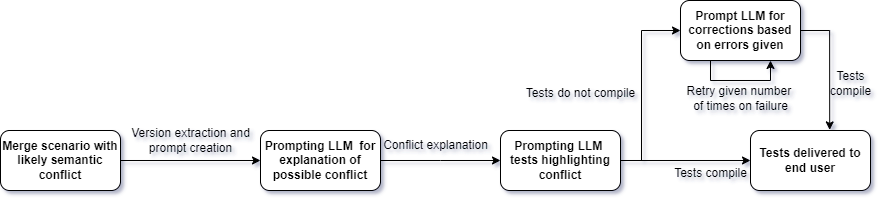
\includegraphics[width=1\linewidth]{figures/tool.png}
    \caption{Functioning pipeline of proposed tool}
    \label{fig:tool}
\end{figure}

\begin{figure}
    \centering
    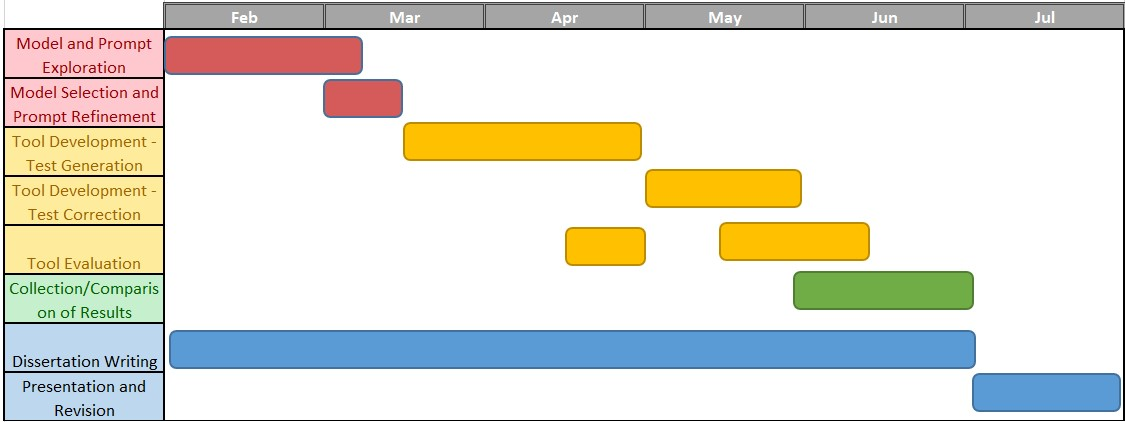
\includegraphics[width=1\linewidth]{figures/gantt.jpg}
    \caption{Gantt diagram of working plan}
    \label{fig:gantt}
\end{figure}